\chapter{Evaluation}

This chapter evaluates the produced framework against the objectives and non-functional requirements outlined in \fullref{ch:objectives}.

\section{Evaluation of objectives}

The framework successfully meets all of the \textit{\textbf{MUST}} requirements outlined:

\begin{itemize}
    \item The framework can determine the best communication channel for the current situation, as shown in \fullref{sec:channel_selection_and_adaption}.
    \item The framework can adapt to its environment, as shown in \fullref{sec:channel_selection_and_adaption}.
    \item The framework can detect and recover from failures in communication, as shown in \fullref{sec:detecting_and_recovering_from_failures}.
    \item The framework uses encrypted communication, with a pre-shared key, as outlined in \fullref{sec:target}.
\end{itemize}

The framework also meets the \textit{\textbf{SHOULD}} requirement:

"The framework can recover from the complete failure of a communication channel", as shown in \fullref{sec:recovering_from_a_communication_channel_failure}.

However the requirement:

"Allow bidirectional communication" is not met, and I think is not possible for the framework to meet this requirement without large refactoring. While the framework does technically allow for bidirectional communication, this is simply limited to a response to a message, not a full conversation. For this system to be capable of bidirectional communication both parties would have to be able to agree on a channel that suits both of their environments, this would require more information to be shared between the parties and a more complex selection algorithm, additionally, this would impose a penalty on the response time of the system to a change in the environment.

The \textit{\textbf{MAY}} requirement:

"[The framework can] handle multiple channels at a time" is also not met, The additional complexity of this requirement is not worth the benefit, although if only direct channels (Ones that go straight from the sender to the receiver) are used, the receiver could reasonably handle multiple channels by tracking the source of the packets, however, this would prevent the use of some channels, such as the TCP Acknowledgement bounce that I utilise in this paper.

\section{Evaluation of non-functional requirements}

\subsection{The effect on covertness of the framework}

The use of multiple channels for communication allows for the framework to adapt to its environment, this is a great benefit to the covertness of the system, it also means that if a channel were to be discovered, for an adversary to extract the information they would have to work out the indexes of the relevant methods, which is a non-trivial task. 

The downside to using multiple channels for communication is that they require protocols, and protocols require a certain degree of structure. Where an adversary is aware of these protocols they could feasibly use them to detect the presence of a covert communication system. This is a problem that is not unique to this framework, but to all covert systems that use protocols.

The reduced covertness of the protocol structure is negligible in comparison to the benefits of multiple channels, as the search domain increases increases with the addition of more channels, and structure is easily mistaken for noise.

Writing a script to identify the channel is simple, however to identify only the channel is much more difficult. It works by searching for the sentinel values in possible channels, in a clear enviornment (where the only traffic between the sender and receiver is the covert channel) this will detect the IP channel with 100\% accuracy, however its false positive rate is much to high to say with certainty that a covert channel exists. This script is available in the appendix at \fullref{sec:warden_py}. The output of running this scipt on a pcap that only lasts for the duration of the covert channel can be seen in figure \ref{fig:warden_output}.

\begin{figure}[H]
    \centering
    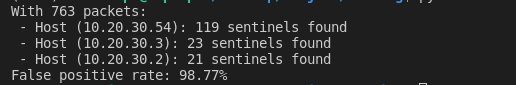
\includegraphics[width=0.7\textwidth]{fig/rudimentary_warden.png}
    \caption{The output of the rudimentary warden script}
    \label{fig:warden_output}
\end{figure}

This script does not represent the true covertness of the channel well, as it assumes the sender knows the channels in the communication, it also assumes the sentinel value, but there is no reason why the sentinel value could not be changed, for example the ones compliment could be applied to all the encoded data, this would mean that the sentinel value would be 0000, which would evade this form of detection.

This type of warden also fails to properly detect the TCP Acknowledgement bounce channel, as the script sees the acknowledgement from the bouncing server, as opposed to the sender, which makes correctly identifying the start/end of a channel incredibly difficult.

For a more accurate warden, it would have to be aware of the following:

\begin{itemize}
    \item The covert methods that are being used.
    \item The sentinel value used.
    \item The index of each method (so it can "follow" the communication).
\end{itemize}

This is a difficult task, but perhaps could be done using a machine learning approach, where the warden is trained on a set of known channels, and then tested on an unknown channel. This would be a good area for future work.

To conclude this evaluation, it is easy to identify a possible covert channel, however it is incredibly hard to identify the channel with certainty, even when the warden has knowledge of the implementation, regardless of wheter this is possible retrospectively, it requires the channel to have already ended to be identifiable, and the solution is not linear in complexity, as the number of channels increase, the number of possible combinations increases exponentially. So the channel cannot be identified with certainty in real-time, or possibly at all, meaning it is incredibly covert.

\subsection{Application of the framework to real-world scenarios}

Issues:

- 

- Julia is wham atm, also see sec below.


\subsection{Capability to add new communication channels}

Adding new channels to the framework is relatively simple, especially for channels that use already-supported protocols (such as IP or TCP), adding new protocols does however require additional work, as the receiver and sender will require a way to represent the protocol as a \inline{Packet} (see \fullref{sec:packet_processing}), and a way to create the packet from a dictionary (see \fullref{sec:sending_packets}) respectively.

While these tasks are not particularly arduous, for somebody unfamiliar with the language they may struggle to understand the codebase, and the lack of documentation regarding the addition of new channels may also be a hindrance.

This is an area that could be improved in future work, by adding documentation and examples or perhaps creating a tool that parses a protocol from a header file and generates the required code.

However, the only way to avoid this problem would be to use a language with support for these packets, such as C, however, this would not come without its problems. For example, C has support for these headers, but it is not as easy to understand or add to the codebase as Julia, conversely, Python is easy to understand and add to, but comes with performance limitations and a lack of portability (Note that Julia does not yet have a stable compilation process, but it is under development).

An implementation of a covert channel can be seen in \fullref{sec:impl_cov_mod}.